% ============================================================================
%  SECTION 9 — EXPERIENCES NUMERIQUES
%  >>> A REMPLIR PAR LE MEMBRE 4 <<<
%
%  Contenu attendu (voir REPARTITION_DETAILLEE.md) :
%    - Validation sur signal synthetique (cf. notebook) : qualite de
%      recuperation vs nombre de vrais coefficients.
%    - COURBE DE CONVERGENCE ISTA vs FISTA (la figure-phare) : illustre
%      empiriquement O(1/k) vs O(1/k^2). Inserer la figure exportee depuis
%      /experiments (style graphique commun du notebook).
%    - Etude de sensibilite : effet de lambda (parcimonie vs fidelite) et du
%      pas t sur la convergence.
%    - Commenter les oscillations de FISTA (lien avec section 6).
%
%  Pour inserer la figure :
%    \begin{figure}[h]\centering
%      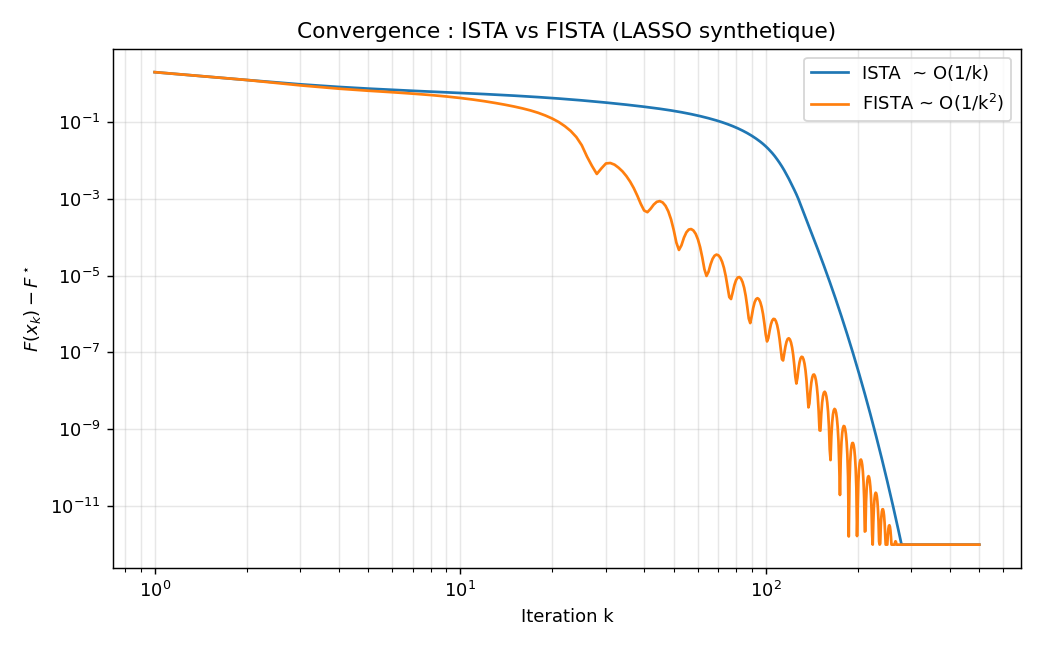
\includegraphics[width=.7\linewidth]{figures/convergence_ista_fista.png}
%      \caption{...}\label{fig:conv}
%    \end{figure}
% ============================================================================
\section{Experiences numeriques}
\label{sec:exp}

% --- [MEMBRE 4] Ecrire la section ici. ---
% TODO
